%% This is file `elsarticle-template-2-harv.tex',
%%
%% Copyright 2009 Elsevier Ltd
%%
%% This file is part of the 'Elsarticle Bundle'.
%% ---------------------------------------------
%%
%% It may be distributed under the conditions of the LaTeX Project Public
%% License, either version 1.2 of this license or (at your option) any
%% later version.  The latest version of this license is in
%%    http://www.latex-project.org/lppl.txt
%% and version 1.2 or later is part of all distributions of LaTeX
%% version 1999/12/01 or later.
%%
%% The list of all files belonging to the 'Elsarticle Bundle' is
%% given in the file `manifest.txt'.
%%
%% Template article for Elsevier's document class `elsarticle'
%% with harvard style bibliographic references
%%
%% $Id: elsarticle-template-2-harv.tex 155 2009-10-08 05:35:05Z rishi $
%% $URL: http://lenova.river-valley.com/svn/elsbst/trunk/elsarticle-template-2-harv.tex $
%%

%%\documentclass[preprint,authoryear,12pt]{elsarticle}

%% Use the option review to obtain double line spacing
%% \documentclass[authoryear,preprint,review,12pt]{elsarticle}

%% Use the options 1p,twocolumn; 3p; 3p,twocolumn; 5p; or 5p,twocolumn
%% for a journal layout:

%% Astronomy & Computing uses 5p
%% \documentclass[final,authoryear,5p,times]{elsarticle}
\documentclass[final,authoryear,5p,times,twocolumn]{elsarticle}

%% if you use PostScript figures in your article
%% use the graphics package for simple commands
%% \usepackage{graphics}
%% or use the graphicx package for more complicated commands
\usepackage{graphicx}
%% or use the epsfig package if you prefer to use the old commands
%% \usepackage{epsfig}

%% The amssymb package provides various useful mathematical symbols
\usepackage{amssymb}
%% The amsthm package provides extended theorem environments
%% \usepackage{amsthm}

\usepackage[,pdftex,pdfpagemode={UseOutlines},bookmarks,bookmarksopen,colorlinks,linkcolor={blue},citecolor={green},urlcolor={red}]{hyperref}
\usepackage{hypernat}

%% Alternatives to hyperref for testing
%\usepackage{url}
%\newcommand{\htmladdnormallinkfoot}[2]{#1\footnote{\texttt{#2}}}
%\newcommand{\htmladdnormallink}[1]{\texttt{#1}}
%\newcommand{\href}[2]{\texttt{#2}}

%% The lineno packages adds line numbers. Start line numbering with
%% \begin{linenumbers}, end it with \end{linenumbers}. Or switch it on
%% for the whole article with \linenumbers after \end{frontmatter}.
%% \usepackage{lineno}

%% natbib.sty is loaded by default. However, natbib options can be
%% provided with \biboptions{...} command. Following options are
%% valid:

%%   round  -  round parentheses are used (default)
%%   square -  square brackets are used   [option]
%%   curly  -  curly braces are used      {option}
%%   angle  -  angle brackets are used    <option>
%%   semicolon  -  multiple citations separated by semi-colon (default)
%%   colon  - same as semicolon, an earlier confusion
%%   comma  -  separated by comma
%%   authoryear - selects author-year citations (default)
%%   numbers-  selects numerical citations
%%   super  -  numerical citations as superscripts
%%   sort   -  sorts multiple citations according to order in ref. list
%%   sort&compress   -  like sort, but also compresses numerical citations
%%   compress - compresses without sorting
%%   longnamesfirst  -  makes first citation full author list
%%
%% \biboptions{longnamesfirst,comma}

% \biboptions{}

\journal{Astronomy \& Computing}

%% Make single quotes look right in verbatim mode
\usepackage{upquote}

\usepackage{upgreek}

\usepackage{color}

\usepackage{listings}

\definecolor{mygreen}{rgb}{0,0.6,0}
\definecolor{mygray}{rgb}{0.5,0.5,0.5}
\definecolor{mymauve}{rgb}{0.58,0,0.82}

\lstset{ %
  backgroundcolor=\color{white},   % choose the background color
  basicstyle=\footnotesize\ttfamily,        % size of fonts used for the code
  breaklines=true,                 % automatic line breaking only at whitespace
  captionpos=b,                    % sets the caption-position to bottom
  commentstyle=\color{mygreen},    % comment style
  escapeinside={\%*}{*)},          % if you want to add LaTeX within your code
  keywordstyle=\color{blue},       % keyword style
  stringstyle=\color{mymauve},     % string literal style
}


% Aim to be consistent, and correct, about how we refer to sections
\newcommand*\secref[1]{Sect.~\ref{#1}}
\newcommand*\appref[1]{\ref{#1}}
\newcommand{\ascl}[1]{\href{http://www.ascl.net/#1}{ascl:#1}}

\begin{document}

\begin{frontmatter}

%% Title, authors and addresses

%% use the tnoteref command within \title for footnotes;
%% use the tnotetext command for the associated footnote;
%% use the fnref command within \author or \address for footnotes;
%% use the fntext command for the associated footnote;
%% use the corref command within \author for corresponding author footnotes;
%% use the cortext command for the associated footnote;
%% use the ead command for the email address,
%% and the form \ead[url] for the home page:
%%
%% \title{Title\tnoteref{label1}}
%% \tnotetext[label1]{}
%% \author{Name\corref{cor1}\fnref{label2}}
%% \ead{email address}
%% \ead[url]{home page}
%% \fntext[label2]{}
%% \cortext[cor1]{}
%% \address{Address\fnref{label3}}
%% \fntext[label3]{}

\title{The General Single-Dish Data Format: A Retrospective\tnoteref{ascl}}
\tnotetext[ascl]{These codes are registered at the ASCL with the code entries \ascl{1503.009} and \ascl{1503.007}.}

%% use optional labels to link authors explicitly to addresses:
%% \author[label1,label2]{<author name>}
%% \address[label1]{<address>}
%% \address[label2]{<address>}

\author[jac]{Tim Jenness\corref{cor1}\fnref{timj}}
\ead{tjenness@lsst.org}
\author[noao]{Elizabeth~B.~Stobie}
\author[nrao]{Ronald~J.~Maddalena}
\author[hp]{Jon~H.~Fairclough}
\author[nrao]{Richard~M.~Prestage}
\author[leiden,imapp]{Remo~P.~J.~Tilanus}
\author[nraocv]{Robert~W.~Garwood}
\author[mrao]{Rachael~Padman}

\cortext[cor1]{Corresponding author}
\fntext[timj]{Present address: LSST Project Office, 933 N.\ Cherry Ave, Tucson, AZ 85721, USA}

\address[jac]{Joint Astronomy Centre, 660 N.\ A`oh\=ok\=u Place, Hilo, HI
  96720, USA}
\address[noao]{National Optical Astronomy Observatory, 950 N Cherry Ave, Tucson, AZ 85719, USA}
\address[nrao]{National Radio Astronomy Observatory, P.O.\ Box 2, Green Bank, WV~24944, USA}
\address[hp]{Hewlett Packard Ltd}
\address[leiden]{Leiden Observatory, Leiden University, PO Box 9513, 2300 RA Leiden, The~Netherlands}
\address[imapp]{Department of Astrophysics,
     Institute for Mathematics, Astrophysics and Particle Physics,
     Radboud University Nijmegen, PO Box 9010, 6500 GL Nijmegen, The~Netherlands}
\address[nraocv]{National Radio Astronomy Observatory,
  Charlottesville, VA~22903-2475, USA}
\address[mrao]{Mullard Radio Astronomy Observatory,
Cavendish Laboratory, University of Cambridge,
JJ~Thomson~Avenue,
Cambridge, CB3~0HE, UK}

\begin{abstract}
%% Text of abstract

The General Single-Dish Data format (GSDD) was developed in the
mid-1980s as a data model to support centimeter, millimeter and submillimeter
instrumentation at NRAO, JCMT, the University of Arizona and IRAM. We
provide an overview of the GSDD
requirements and associated data model, discuss the implementation
of the resultant file formats, describe its usage in the observatories and
provide a retrospective on the format.

\end{abstract}

\begin{keyword}
%% keywords here, in the form: keyword \sep keyword

%% MSC codes here, in the form: \MSC code \sep code
%% or \MSC[2008] code \sep code (2000 is the default)

data formats \sep
submillimeter: general \sep
history and philosophy of astronomy

\end{keyword}

\end{frontmatter}

% \linenumbers

%% Journal abbreviations
\newcommand{\mnras}{MNRAS}
\newcommand{\aap}{A\&A}
\newcommand{\aaps}{A\&AS}
\newcommand{\pasp}{PASP}
\newcommand{\apj}{ApJ}
\newcommand{\apjs}{ApJS}
\newcommand{\qjras}{QJRAS}
\newcommand{\an}{Astron.\ Nach.}
\newcommand{\ijimw}{Int.\ J.\ Infrared \& Millimeter Waves}
\newcommand{\procspie}{Proc.\ SPIE}
\newcommand{\aspconf}{ASP Conf. Ser.}

%% Applications

%% Misc

%% Links


%% main text

\section{Introduction}

In the late 1970s and early 1980s millimeter and submillimeter
single-dish astronomy was undergoing a significant period of growth \citep[see
e.g.,][]{2013ASSP...37...39R} with the NRAO 12-m telescope leading the
way \citep[see e.g.,][]{2005ASSL..323.....G} and with multiple
observatories being developed such as the IRAM 30-m
\citep{1981MitAG..54...61B}, the 15-m James Clerk Maxwell Telescope
\citep[JCMT;][]{1985ESOC...22...63H}, the 10-m Sub-Millimeter
Telescope \citep[SMT;][]{1985ESOC...22...71W}, the 15-m Swedish ESO
Submm Telescope \citep[SEST;][]{1985ESOC...22...25D}, and the Caltech
Submillimeter Observatory \citep[CSO;][]{1988BAAS...20..690P}. In this
environment it was recognized by some institutions that the ability
for data taken on one telescope to be reduced and analyzed by the
software written at another telescope would be extremely useful and
could lead to significant savings on software development effort.

At this time the Flexible Image Transport System
\citep[FITS;][]{1981A&AS...44..363W} was considered mainly
suitable as a means of exchanging image data using tapes
\citep{1980SPIE..264..298G}. The FITS standard, which then
lacked the capability to use binary tables and could only store a
single ASCII table per file, was not deemed an
efficient format to store complex mm/submm time-series and
spectral-line data from single-dish telescopes that usually required
many sets of tabular data.

The General Single Dish Data format (GSDD) was developed in the 1980s
to solve the data processing and acquisition requirements of the NRAO,
IRAM, University of Arizona and JCMT observatories.  Initial
discussions between NRAO 12m and IRAM staff began in 1983, and
subsequently included JCMT representatives. At around this same time,
however, IRAM started development of the Continuum and Line Analysis
Single-dish Software
\htmladdnormallinkfoot{\textsc{class}}{http://www.iram.fr/IRAMFR/GILDAS}
\citep[][\ascl{1305.010}]{2005sf2a.conf..721P} data reduction package,
and they did not follow up on the GSDD initiative.\footnote{The
  authors have been unable to find anyone from IRAM or the University
  of Arizona that recalls the GSDD discussions and can provide
  information from their side. JCMT and NRAO documents confirm the
  additional parties but no meeting minutes are available. An IRAM
  memo from January 1983 indicates they were strongly in favor of a
  FITS variant called IRAM Disk-oriented FITS (IDFITS) that supported
  VAX floating point, array header keywords, variable length headers
  (up to 80 characters) and \texttt{CONTINUE} cards and stored the
  data in separate files from the header information.}  The GSDD
format, agreed in 1986 \citep[see e.g.,][]{mtdn84,1987NRAO30},
consisted of a data model for specifying centimeter, millimeter and
submillimeter observations (continuum and spectral-line
instrumentation) and a specification of how the bytes would be
represented on disk.  The format was described in both JCMT technical
notes \citep{mtdn84,mtdn85,SUN229} and an NRAO Newsletter article
\citep{1987NRAO30}, but a formal definition of the format was not
published in the literature. In this article we present the first
joint NRAO/JCMT description of the model and provide a retrospective
on the history and usage of the format.

\section{Data Model}

To allow interoperability of data files between differing
observatories it was important to develop a shared data model,
taking particular care to allow simple interchange of reduced spectra
between software packages. Reduced data has fewer instrument-specific
variations and was deemed to be the simplest first step, requiring
sufficient metadata to specify the coordinates of the spectrum on the
sky, the frequency scale and the calibrated
units of the spectrum.

\begin{table*}
\caption{Model classes used by the various GSDD models.}
\label{tab:classes}
\begin{center}
\begin{tabular}{lll}
\hline
Class number & NRAO Meaning & JCMT meaning\\ \hline
1         & Basic Information                                                 &    Identity Parameters        \\
2         & Pointing Parameters                                               &    Time Parameters            \\
3        & Observing Parameters                                               &    Position Parameters        \\
4          & Positions                                                        &    Pointing Parameters        \\
5      & Environment                                                          &    Environment Parameters     \\
6        & Map Parameters                                                     &    Mapping Parameters         \\
7          & Data Parameters                                                  &    Velocity Parameters        \\
8       & Engineering Parameters                                              &    Engineering Parameters   \\
9           & Telescope Dependent Parameters                                  &    Data Parameters            \\
10       & Open Data Reduction Parameters                                     &   Receiver Parameters         \\
11       & Phase Block                                                        &   Phase Control Table         \\
12        & Descriptor Block for Each Receiver Channel                        &   Phase Value Table           \\
13       & Spectral Values                                                    &   Phase Timing Table          \\
14          & ---                                                             &   Data Value Table            \\
15           & ---                                                           &   Pointing History            \\
55                                        & ---                               &   Inclinometry                \\
\hline
\end{tabular}
\end{center}
\end{table*}

When designing the model related items were grouped into numbered
classes and the parameter name was prefixed by that class number. The
class groupings are shown in Table~\ref{tab:classes} and indicate that
there was some disagreement in naming convention after the standard
was agreed.\footnote{Given the agreement in item names, it is likely
  that the class names are due to a documentation error at JCMT rather
  than an implementation error at JCMT.} Despite this documented
difference in class naming \citep{mtdn85}, 71 data items were named
consistently in the NRAO and JCMT implementations\footnote{72 if the
telescope-specific \texttt{C9OT}, Observing Tolerance, item is included which was present in the
NRAO 12m definition and at JCMT but not used for Green Bank} and those are
detailed in Table~\ref{tab:core}. For example \texttt{C3DAT} referred
to the UT date of the observation, \texttt{C1SNO} the scan number,
and \texttt{C7VR} the source radial velocity.

At the JCMT these GSDD names (known locally as the ``NRAO'' names)
were written to disk files but were mapped to local equivalents in
the acquisition computers. For example \texttt{C12RF}, the rest
frequency, mapped to \texttt{FE\_NUREST} in the acquisition system and
was equivalent to the \texttt{RESTFREQ} FITS keyword. A full list of
the equivalences for JCMT can be found in \citet{SUN229}.

One key feature of the GSDD design was that some classes were
explicitly reserved for local use. Class 9 was used for telescope
dependent parameters and the defined set differed between Green Bank
and the 12m with JCMT adopting a single item, \texttt{C9OT} from the 12m.

\begin{table*}[t]
\centering
\caption{Core components of GSDD data model present in both NRAO and
  JCMT implementations.}
\label{tab:core}
\begin{tabular}{|lp{1.5in}|lp{1.5in}|lp{1.5in}|}
\hline
\textbf{C1BKE} & Backend & \textbf{C4CSC} & Code for coordinate system & \textbf{C6YGC} & Starting Y grid position \\
\textbf{C1DP} & Precision & \textbf{C4EDC} & Epoch declination / Declination of date & \textbf{C6YNP} & Number of Y grid points \\
\textbf{C1OBS} & Observer Initials / Observer Name & \textbf{C4EL} & Elevation at C3UT & \textbf{C7BCV} & Bad channel value \\
\textbf{C1ONA} & Observer name & \textbf{C4EPH} & Epoch of coordinates & \textbf{C7CAL} & Calibration type \\
\textbf{C1PID} & Project ID & \textbf{C4ERA} & Epoch Right Ascension & \textbf{C7OSN} & Calibration scan/observation number \\
\textbf{C1RCV} & Frontend & \textbf{C4GB} & Galactic Latitude & \textbf{C7VC} & Velocity correction \\
\textbf{C1SNO} & Scan number / Observation number & \textbf{C4GL} & Galactic Longitude & \textbf{C7VR} & Radial velocity of source \\
\textbf{C1STC} & Type of observation & \textbf{C4RX} & Reference X position & \textbf{C7VRD} & Velocity definition code \\
\textbf{C1TEL} & Telescope name & \textbf{C4RY} & Reference Y position & \textbf{C8AAE} & Aperture efficiency \\
\textbf{C2FL} & EW focus & \textbf{C4SX} & Source X & \textbf{C8ABE} & Beam efficiency \\
\textbf{C2FR} & Radial focus & \textbf{C4SY} & Source Y & \textbf{C8EF} & Forward spillover \& scattering efficiency \\
\textbf{C2FV} & NS focus & \textbf{C5AT} & Ambient Temperature & \textbf{C8EL} & Rear spillover \& scattering efficiency \\
\textbf{C2ORI} & Secondary orientation & \textbf{C5DP} & Dew point & \textbf{C8GN} & Antenna gain \\
\textbf{C2XPC} & Az/RA pointing correction & \textbf{C5IR} & Refractive index & \textbf{C11VD} & Phase table names \\
\textbf{C2YPC} & El/Dec pointing correction & \textbf{C5MM} & Atmospheric vapor pressure & \textbf{C12BW} & Bandwidth \\
\textbf{C3CL} & Length of cycle & \textbf{C5PRS} & Atmospheric pressure & \textbf{C12CF} & Observed frequency \\
\textbf{C3DAT} & UT date (YYYY.MMDD format) & \textbf{C5RH} & Relative humidity & \textbf{C12CT} & Calibration temperature \\
\textbf{C3LST} & LST at start & \textbf{C6DX} & Delta X offset & \textbf{C12FR} & Frequency resolution \\
\textbf{C3NRC} & Number of rx/backend channels & \textbf{C6DY} & Delta Y offset & \textbf{C12RF} & Rest frequency \\
\textbf{C3NSV} & Number of switching/phase table variables & \textbf{C6FC} & Reference frame coord code & \textbf{C12RST} & Reference system temperature \\
\textbf{C3PPC} & Number of phases per cycle & \textbf{C6MSA} & Scanning angle & \textbf{C12RT} & Receiver temperature \\
\textbf{C3SRT} & Integration time & \textbf{C6NP} & Number of grid points & \textbf{C12SST} & Source system temperature \\
\textbf{C3UT} & UT hour of observation / UT1 & \textbf{C6XGC} & Starting X grid position & \textbf{C12WO} & Water opacity \\
\textbf{C4AZ} & Azimuth at C3UT & \textbf{C6XNP} & Number of X grid points &   &   \\
\hline
\end{tabular}
\end{table*}

The NRAO implementation, not including class 9, includes 26 items not
found in the JCMT version. The reasons they were not adopted at JCMT
are:

\begin{description}

\item[\texttt{C1DLN} \texttt{C1HLN}] are not needed at JCMT
  because the length of the header region and the length of the data
  region are encoded in the file format design.

\item[\texttt{C1SNA}] is the source object name and exists as two separate
  items at JCMT, \texttt{C1SNA1} and \texttt{C1SNA2}, to allow the
  object name to be specified in two parts or with an alternative name
  given. \texttt{C1SNA1} is the primary source name and is equivalent
  to the \texttt{OBJECT} FITS keyword. Historically the alternate or
  secondary part of the name was rarely used at JCMT so the name
  change, in hindsight, turned out to be unnecessary.

\item[\texttt{C2PC}] was used at NRAO to specify a four-element
  secondary pointing correction. The JCMT version specifies this as
  four discrete scalar items, \texttt{C2PC1} to \texttt{C2PC2}, rather
  than using an array.

\item[\texttt{C2UXP} \texttt{C2UYP}] are the user Az/RA and El/Dec
  pointing corrections in arcsec but at JCMT these were simply called
  \texttt{UAZ} and \texttt{UEL} with no class prefix and no RA/Dec
  equivalent.

\item[\texttt{C4DO}] is a three-element array labeled ``Descriptive
  Origin'' describing the position and angle of the coordinate system
  defined by the observer. At JCMT this was implemented as three
  distinct items \texttt{C4DO1} through \texttt{C4DO3} and specified
  the observing cell size and position angle with respect to local
  vertical. There was disagreement between NRAO and JCMT on the
  definition here as the three elements at NRAO referred to the
  horizontal and vertical position and the position angle with respect
  to the horizontal axis. Documents and source code from JCMT indicate
  these items were not used and are duplicates of items \texttt{C6DX},
  \texttt{C6DY} and \texttt{C6MSA}.

\item[\texttt{C4IX} \texttt{C4IY}] are the coordinates of the
  telescope as measured by the encoders. This information was not
  recorded by JCMT.

\item[\texttt{C6XZ} \texttt{C6YZ}] specify the position of the map
  origin. These coordinates are not stored at JCMT as the map is
  defined in terms of offsets from the specified tracking centre.

\item[\texttt{C7FW}] is the beam full width at half maximum in arcsec
  at NRAO but at JCMT the item used is \texttt{C7HP} and most JCMT data
  files do not seem to set it.

\item[\texttt{C11*}] is nominally the phase block. At JCMT
  \texttt{C11VD} specifies the names of the columns of the phase table
  information stored in \texttt{C11PHA} where the dimensionality is
  specified by \texttt{C3NSV} (number of phase table variables) and
  \texttt{C3PPC} (number of phases per cycle). NRAO use \texttt{C11VV}
  to store the values of a single switch state and the phase table is
  \texttt{C11PHT}.

\item[\texttt{C12IT} \texttt{C12NI} \texttt{C12SPN}] indicate the integration time,
  the number of integrations and the starting point in the data block
  for each receiver channel. {\color{red} I guess ``receiver channel''
    is the equivalent of a JCMT backend section?}. JCMT data require
  that each backend section has the same integrations, requiring no
  keywords to indicate this.

\item[\texttt{C12ST} \texttt{C12RMS}] are the computed source
  temperature and the RMS value. The JCMT online observing system did
  not calculate this.

\item[\texttt{C12SP}] is a description of the polarization type and
  angle encoded in an eight character field. This item was not used at
  JCMT.

\item[\texttt{C12RP} \texttt{C12X0} \texttt{C12DX}] {\color{red} No
    idea what X-axis means in this context.}

\item[\texttt{C12WT}] is the water temperature. Not measured directly
  at JCMT during this period.

\item[\texttt{C12OO} \texttt{C12OT}] is the oxygen opacity and
  temperature. Not measured at JCMT.

\end{description}

Additionally, whilst JCMT did use \texttt{C5IR} to report the mean
refractive index, the JCMT format also stored the three refraction constants
defined in the model \citep{mtin26} as \texttt{C5IR1}, \texttt{C5IR2}
and \texttt{C5IR3}.

\section{National Radio Astronomy Observatory}


The 12-m Telescope was upgraded to write GSDD format data in the
summer of 1986 \citep{tcus23,1987NRAO30}; requiring that the data
analysis system was also updated to understand it.

In 1988 the NRAO decided for a number of reasons to unify the data
reduction systems for its single-dish telescopes: the Tucson 12-m, and
the Green Bank 300\,ft and 140\,ft telescopes.  At the time all three
telescopes used what looked like a very similar data reduction system,
the People Oriented Parsing Service \citep[POPS;][]{1982POPS}
But, at the code level the applications in Green Bank
and Tucson had been diverging rapidly since the early 1980's,
essentially due to the different computer architectures at the two
sites (early 1970's Modcomps in Green Bank and mid-1980 DEC VAX's in
Tucson).  The NRAO wanted to reduce maintenance costs as different
staff were needed to maintain and develop each version.  The NRAO was
also migrating to Unix-based (primarily Sun) computers, a change that
would require major modifications to POPS. The unified analysis system, UniPOPS
\citep[][\ascl{1503.007}]{UNIPOPS}, was started in early 1989 and first released to users in early
1991 \citep{1991BAAS...23..535V}.  Although the 300\,ft collapsed in
1988 \citep{1990BAAS...22..487V}, and the 140\,ft was
decommissioned for astronomy in 1999, UniPOPS is still in use today at
some level by the University of Arizona who took over the running of
the 12-m telescope in 2004.

Since the majority of the FORTRAN code that was modified to create
UniPOPS came from the 12-m version of POPS, the UniPOPS developers
decided that UniPOPS would also inherit with little modification the
underlying data structure and export formats of the 12-m version of
POPS.  The UniPOPS data structure is, thus, identical to the POPS Data File
(PDFL) export file format, which was the 12-m version of GSDD.  Adapting 140\,ft
and 300\,ft data to use the GSDD format was
relatively easy, good evidence that GSDD was indeed a rather versatile
and useful standard.

Two modifications were made to the PDFL files when they were
incorporated into UniPOPS, solely to boost the performance of the
system.  The binary representation was changed from that of the DEC
architecture to that of Sun workstations.  And, the index that was at
the start of a PDFL file was extended to include such items as the sky
location and observing frequency so as to make it possible to do more
efficient searches through the data.  To distinguish the UniPOPS
Sun-specific exported files from VAX PDFL files, the NRAO developers
changed the name of the export format to Single Dish Data (SDD) format.
Other than a modification that expanded the capabilities of the index
section of the NRAO SDD files, the SDD format adopted for UniPOPS
(Fig.~\ref{fig:nraosdd}) remained unchanged until UniPOPS was retired
at the NRAO in the mid-2000's.

\begin{figure}[t]
\begin{center}
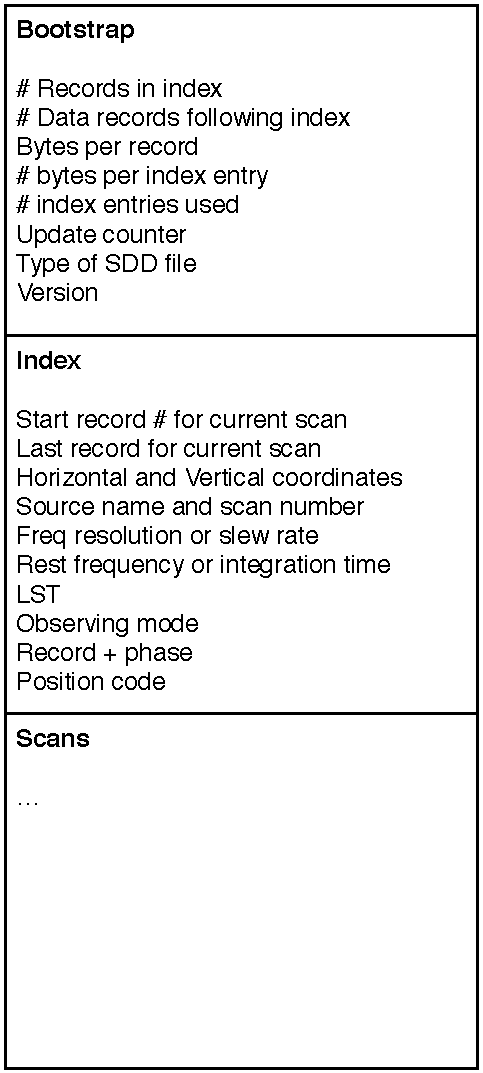
\includegraphics[width=0.5\columnwidth]{sdd-file-layout}
\end{center}
\caption{Layout of a UniPOPS data file. The concepts are similar to
  those used in the GSD format (Fig.~\ref{fig:jcmtgsd}). The bootstrap
  field describes the basic layout of the file and the index indicates
  where each of the scans are located in the file. A key difference
  between GSD and SDD is that GSD contains a single observation
  whereas an SDD file contains many observations for a single science
  program.}
\label{fig:nraosdd}
\end{figure}

By the late 1980's, users of the NRAO telescopes were very interested
in seeing a FITS format implemented for the NRAO's single-dish
telescopes (see \S\,\ref{sec:sdfits}). By the mid 1990's,
UniPOPS could export and import data in Single Dish FITS (SDFITS) and
SDD formats, as well as many
of the historical NRAO formats.  The NRAO found that very few users
went away with SDFITs format; most took home SDD files.  Since
users were installing UniPOPs on their home computers, they probably
found transporting SDD files more convenient than using
SDFITS files.  It was probably very rare that a UniPOPS SDD file was
imported into another analysis system.  For example, a separate
utility was developed that would prepare data files that could be
imported into the {\textsc CLASS} package.
Furthermore, when SDFITs was released, few FITS readers at the
time could actually usefully import binary tables.  Thus, we suspect
that frequent observers grew into the habit of avoiding SDFITS files.

\section{James Clerk Maxwell Telescope}

\subsection{Requirements}

During the development of the JCMT software libraries at the Mullard
Radio Astronomy Observatory, a number of options were considered for
the raw data file format.  Two obvious options were available in the
astronomical community in the form of the Flexible Image Transport System
\citep[FITS;][]{1981A&AS...44..363W} and the Starlink Hierarchical
Data System \citep[HDS;][\ascl{1502.009}]{1982QJRAS..23..485D,2015HDS}.

FITS was discounted as the primary data format because of the large
amount of overhead required to format the header information when
writing files and the inability of the format (at that time) to store
more than one
data array or table in a file. FITS files at the time were not capable
of storing binary tables and ASCII tables were all that was possible
\citep{1988A&AS...73..365H}. It was also felt that the DEC Backup
Utility was more reliable for transport and archiving than using a
FITS tape format. Whilst the FITS community would
eventually support multiple data arrays and binary tables, it was not
possible to wait for that to happen.

HDS was discarded for I/O efficiency reasons and the inability for the
entire file to be mapped into memory in one operation. Additionally it
was felt that the HDS library API required too many calls to do simple
tasks. One further option was to use the NRAO 12-m file format (PDFL)
but that also suffered from serious I/O issues and could not be used
on the acquisition hardware initially targeted for JCMT.

The computer used during testing and commissioning in 1985/86 was a
VAX 11/730 which had severe performance limitations. This was upgraded
to a MicroVAX just before operations started at JCMT in 1987 but
performance was the key design driver: the control system was required
to minimize the overheads in data capture and therefore maximize the
observing time.

Given the performance requirements for the JCMT data acquisition
system it was important that a file could be mapped using VMS system
services as a Global Section to allow other applications to get read
access to the contents of the file whilst it was being written.  This
led to the JCMT implementation of the library being known as the
Global Section Datafile System \citep[GSD;][]{mtin33}\footnote{In retrospect,
the similarity of acronyms between GSD and GSDD -- two quite separate
concepts -- was rather unfortunate. The
  naming of the library as GSD eventually led to JCMT users referring
  to the files as being of ``GSD format'' rather than ``GSDD
  format''.}.

These requirements led to a new format being devised and an associated
I/O library which used the GSDD data model, with the file format design
influenced by the NRAO approach to a self-describing GSDD
implementation and also the concept of an ``in memory data base
management system'' from the \texttt{MON} library being used in the
JCMT control system.  JCMT adopted the GSDD data model in the hope
that downstream the data reduction systems could be compatible through
the shared metadata conventions.

\subsection{File Format Design}

\begin{figure}
\begin{center}
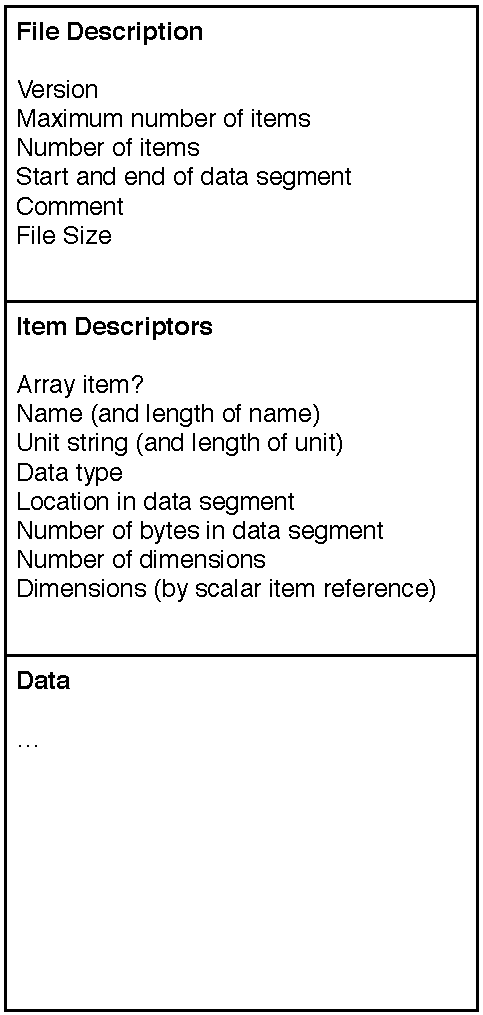
\includegraphics[width=0.5\columnwidth]{gsd-file-layout}
\end{center}
\caption{Layout of a JCMT GSD data file. The file descriptor indicates
where the data starts and the number of items in the data. The item
descriptors describe each of those items and where they are located in
the data segment.}
\label{fig:jcmtgsd}
\end{figure}

The layout of a JCMT GSD format file is shown in
Fig.~\ref{fig:jcmtgsd} \citep[see also][]{mtdn84}. The file is split
into three segments: the file descriptor, the item descriptors and the
data itself. The file descriptor contains a general description of the
file indicating its version, the number of items written and the
position of the data array. The item descriptors define each of the
items in terms of the label and units and the position in the data
array. For array items (GSDD supported up to 5 dimensions), the
identity of each dimension is specified in terms of the number of a
scalar item. This allows the label and unit to be associated with each
dimension of an array item in addition to the size of the
dimension. For example, the \texttt{C11PHA} array entry in a JCMT DAS
spectrum \citep{1986SPIE..598..134B} is dimensioned according to the
scalar items \texttt{C3NSV} and \texttt{C3PPC}, with a negative number
of dimensions indicating that an item is a scalar that defines an
array dimension.

The JCMT format implementing GSDD supports the standard Fortran data
types of byte, word, logical, integer, real, double and character
strings, and uses VAX floating point format \citep[see][for more
information on VAX floating point format]{Payne:1980:VFP:641845.641849}. To simplify the format,
character strings have a fixed size of 16 characters, item names are
fixed at 15 characters and unit strings are fixed at 10
characters. The format supported the concept of a ``null'' value by
reserving the most negative value of each data type for that purpose
(using a single space as the null character value and false as the
null logical value). Additionally, the JCMT GSD library supported data
type conversion, allowing a user to request a value in a different
type to how it was stored natively in the file.

\subsection{Format Usage}

The JCMT took data in the GSDD format for all instruments (heterodyne
and continuum) from the telescope commissioning (circa 1986) to the
delivery of SCUBA in 1996 \citep{1999MNRAS.303..659H}. The GSDD format
continued to be used for heterodyne instruments until the delivery of
the new ACSIS correlator in 2006 \citep{2009MNRAS.399.1026B}. SCUBA
and the new instruments wrote data in the Starlink extensible
\emph{N}-dimensional Data Format \citep[NDF;][]{2015NDF}, although
SCUBA's data model did not exactly match that used for ACSIS and
SCUBA-2 \citep{2013MNRAS.430.2513H} data. The GSD data access library
was a VAX-specific library \citep{1986QJRAS..27..675.,mtdn84} written
in Fortran and making extensive use of VAX system calls. When
the last instrument moved off of the VAX/VMS data acquisitions computers
the format could no longer be used and was retired.

The GSDD data files are archived at the Canadian Astronomy Data
Centre and approximately 440\,000 GSD format files are in the
archive, totalling approximately 30\,GB. In order to access these data
files on a Unix system a new read-only version of the GSD library was
written in C \citep[][\ascl{1503.009}]{SUN229} and integrated into the standard data
reduction tools SPECX \citep[][\ascl{1310.008}]{SPECX,1990JCMTP...9...25P}, COADD
\citep[][\ascl{1411.020}]{COADD}  and JCMTDR
\citep[][\ascl{1406.019}]{SUN132}.  The GSD format is relatively
simple and the main complication in the new C (and later pure Java)
implementations was the conversion of VAX floating point format to
IEEE format. Furthermore, computers were sufficiently more powerful
by the time the Unix version was written that there was no need to use
memory mapping; the entire contents of a file is read into memory.
GSD was solely used as a data acquisition format at JCMT, with there
being one application on the VAX to enable the editing of contents if
there was a need to fix some metadata. Data reduction applications
never wrote data out in GSD format and the Unix port of the library
did not have the ability to write a GSD file.
A Perl interface to the Unix C GSD library \citep{1999ASPC..172..494J}
was implemented to allow the preview of spectra for remote observers
when doing flexible scheduling \citep{1997ASPC..125..401J}.

There is currently a plan at the Joint Astronomy Centre to convert the
heterodyne files to the modern ACSIS format \citep{OCS_ICD_022} such that they can be
reduced using the standard JCMT data reduction pipelines
\citep{2015ACSISDR,2008ASPC..394..565J}. The standard SMURF data reduction application
(\ascl{1310.007}\nocite{2013ascl.soft10007J}) contains the ability to
read GSD files and migrate them to the modern format \citep{SUN259}.

The GSD files from the earlier continuum instruments, such as UKT14
\citep{1990MNRAS.243..126D}, will remain in the archive although they
will not be visible in the JCMT Science Archive \citep{2015Economou}.


\section{Retrospective}

GSDD has had a mixed history and in this section we look back on the
good and bad of GSDD.

\subsection{The hidden standard}

The key failure of GSDD was that most of the users of the format did
not realize that it was a standard and therefore there was no
impetus for people to continue to communicate as systems
evolved. The initial developers of the JCMT system were not the people
maintaining the acquisitions software in Hawaii; the lead developer of
the 12m GSDD system left NRAO before the end of the 1980s.
Interviewing people from NRAO and JCMT following the
respective implementations of GSDD compatible systems, it was very rare
for anyone to remember that there was an intent for a standard to be
in place. As can be seen from the evolution of the JCMT class names
and the divergence of data models, items were added to the respective
data formats without any communication between the nominal GSDD
partners. 12-m development continued with tweaking of the acquisition
and reduction formats independently.  As the GSDD model evolved, the
NRAO implementation resulted in 24 items that are not present in the
JCMT implementation (not including the classes explicitly specified to
be locally defined), and 154 items that are defined by JCMT but not
defined by NRAO.

The goal of unified data reduction software understanding GSDD never
materialized. Indeed, interoperability usually occurred, if at all, by exporting
the files into a completely different format that could be understood
by \textsc{class}.

In conclusion, it is impossible for a standard to survive as a standard
if no-one knows they are using a standard.

\subsection{Embrace Flexibility}

A major advantage of GSDD is that the standard actually allowed sites
to alter the format and data model as they saw fit.  But, sites had to
follow some minor rules in order to guarantee that any other site's
GSDD reader could still manage the files.  Such rules as: do not touch
the pre-defined keywords (which were to have predefined byte sizes and
were always to be in a certain order at the start of a class), you are
free to add new keywords to any class but only at the end of the
pre-defined section of each class, modify class 9 for your particular
telescope, modify class 10 as convenient, and be sure to
use the well-defined pre-amble to designate the byte at which every
class begins.  We maintain that GSDD was actually a very good
implementation for its time because these rules could be easily
adhered to while simultaneously giving sufficient versatility to each
telescope.

\subsection{Clear separation of model from file format}

Whether by accident or design, the GSDD standard resulted in multiple
software implementations writing the data to disk in different formats
and using different techniques. The JCMT GSD format was never written
on anything other than a VAX but the NRAO format migrated from PDFL to
SDD. GSDD benefited by explicitly defining the data model for
single-dish observing distinct from bytes on the disk.

\subsection{A success apart}

Despite the lack of communication between implementors and the drift
in specifications, the GSDD format itself can be thought of as a
success when the uses of the format are looked at independently. The JCMT GSD
format was used for many years and files in this format are still
available. The related format continues to be used at the 12-m Telescope.


\subsection{Feeder for SDFITS}
\label{sec:sdfits}

GSDD was a very early attempt for independently run observatories to
agree on a shared data model. The goals of true interoperability of
raw telescope data amongst multiple data reduction software packages
was an important goal that was ahead of its time. Arguably they key
outcome of GSDD was that it motivated people to work together towards
a shared data format based on FITS. The GSDD experience fed in to a
1989 workshop held at Green Bank in late
1989\footnote{\url{http://fits.gsfc.nasa.gov/dishfits/dishfits.8910}}
that discussed how the community could migrate to a
single-dish FITS format. This was a key motivator for the adoption
into the FITS standard of binary tables \citep{1995A&AS..113..159C}
and ultimately led to the SDFITS standard \citep{2000ASPC..216..243G}.

\subsection{Communication}

A failing of GSDD is that when developers had real, practical reasons
to break a rule (e.g., needing a double precision word for a
pre-defined keyword when the standard required single precision, a
string needing 32 char instead of 16, changing the byte representation
from that of a VAX to IEEE), a forum had not been set up that could
negotiate modifications to the standard.  This is unlike the FITS
world where revisions to the definition have to pass through a
standards group.  A key lesson is that when a first-class standard is
set up, the agreement should go beyond the expectation that ad hoc
conversations between staff at different observatories are a
sufficient means of keeping the standard viable.

The JCMT GSD library was documented and stable and the UK had the
Starlink Project \citep{1982QJRAS..23..485D} to publish the software
and data files to the UK community. Access to that network from other
countries, such as the US, was problematic, and hindered the spread of
the software and prevented take up. Fears of lack of support also
drive people to create their own in-house solutions.

Today, 30 years on, the Internet and the culture of open-source
development make that much less likely and a good idea has a better
chance of surviving and growing.

\section{Conclusions}

The GSDD data model was used at NRAO and JCMT for many years
but failed in its original goal of unifying single dish millimeter
astronomy and simplifying data reduction software reuse. As data
reduction packages have evolved it has become clear that the most
important aspect of such packages is format conversion such that the
software can map the external data model to an internal data model. It
is simply too hard to motivate individual observatories to target a
global standard for raw data. Interoperability of reduced data
products has significantly improved since the mid-1980s such that
there is a general expectation that reduced data cubes will be
viewable in general tools.


\section*{Acknowledgments}

The National Radio Astronomy Observatory is a facility of the National
Science Foundation operated under cooperative agreement by Associated
Universities, Inc.
The James Clerk Maxwell Telescope has historically been operated by
the Joint Astronomy Centre on behalf of the Science and Technology
Facilities Council of the United Kingdom, the National Research
Council of Canada and the Netherlands Organisation for Scientific
Research. We thank Thomas Folkers and Harvey Liszt for useful
discussions on GSDD. This research has made use of NASA's Astrophysics
Data System.

The source code for the JCMT GSD library (C, Perl wrapper, and Java)
and the source code for UniPOPS are available from
Github\footnote{UniPOPS at \url{https://github.com/nrao/UniPOPS} and JCMT
  GSD at \url{https://github.com/Starlink/starlink}}
and both are distributed under the Gnu General Public Licence. The
JCMT GSD library is distributed as part of the Starlink software
collection \citep[see e.g.,][\ascl{1110.012}]{2014ASPC..485..391C}.

%% References
%%
%% Following citation commands can be used in the body text:
%%
%%  \citet{key}  ==>>  Jones et al. (1990)
%%  \citep{key}  ==>>  (Jones et al., 1990)
%%
%% Multiple citations as normal:
%% \citep{key1,key2}         ==>> (Jones et al., 1990; Smith, 1989)
%%                            or  (Jones et al., 1990, 1991)
%%                            or  (Jones et al., 1990a,b)
%% \cite{key} is the equivalent of \citet{key} in author-year mode
%%
%% Full author lists may be forced with \citet* or \citep*, e.g.
%%   \citep*{key}            ==>> (Jones, Baker, and Williams, 1990)
%%
%% Optional notes as:
%%   \citep[chap. 2]{key}    ==>> (Jones et al., 1990, chap. 2)
%%   \citep[e.g.,][]{key}    ==>> (e.g., Jones et al., 1990)
%%   \citep[see][pg. 34]{key}==>> (see Jones et al., 1990, pg. 34)
%%  (Note: in standard LaTeX, only one note is allowed, after the ref.
%%   Here, one note is like the standard, two make pre- and post-notes.)
%%
%%   \citealt{key}          ==>> Jones et al. 1990
%%   \citealt*{key}         ==>> Jones, Baker, and Williams 1990
%%   \citealp{key}          ==>> Jones et al., 1990
%%   \citealp*{key}         ==>> Jones, Baker, and Williams, 1990
%%
%% Additional citation possibilities
%%   \citeauthor{key}       ==>> Jones et al.
%%   \citeauthor*{key}      ==>> Jones, Baker, and Williams
%%   \citeyear{key}         ==>> 1990
%%   \citeyearpar{key}      ==>> (1990)
%%   \citetext{priv. comm.} ==>> (priv. comm.)
%%   \citenum{key}          ==>> 11 [non-superscripted]
%% Note: full author lists depends on whether the bib style supports them;
%%       if not, the abbreviated list is printed even when full requested.
%%
%% For names like della Robbia at the start of a sentence, use
%%   \Citet{dRob98}         ==>> Della Robbia (1998)
%%   \Citep{dRob98}         ==>> (Della Robbia, 1998)
%%   \Citeauthor{dRob98}    ==>> Della Robbia


%% References with bibTeX database:

\bibliographystyle{model2-names-astronomy}
\bibliography{acgsd}

%% Authors are advised to submit their bibtex database files. They are
%% requested to list a bibtex style file in the manuscript if they do
%% not want to use model2-names.bst.

%% References without bibTeX database:

% \begin{thebibliography}{00}

%% \bibitem must have one of the following forms:
%%   \bibitem[Jones et al.(1990)]{key}...
%%   \bibitem[Jones et al.(1990)Jones, Baker, and Williams]{key}...
%%   \bibitem[Jones et al., 1990]{key}...
%%   \bibitem[\protect\citeauthoryear{Jones, Baker, and Williams}{Jones
%%       et al.}{1990}]{key}...
%%   \bibitem[\protect\citeauthoryear{Jones et al.}{1990}]{key}...
%%   \bibitem[\protect\astroncite{Jones et al.}{1990}]{key}...
%%   \bibitem[\protect\citename{Jones et al., }1990]{key}...
%%   \harvarditem[Jones et al.]{Jones, Baker, and Williams}{1990}{key}...
%%

% \bibitem[ ()]{}

% \end{thebibliography}

\end{document}

%%
%% End of file `elsarticle-template-2-harv.tex'.
